%---------- INICIO DEL PREÁMBULO ----------
\documentclass[12pt,a4paper]{article}

% --- Idioma y codificación ---
\usepackage[utf8]{inputenc}      % permite escribir tildes/ñ directamente
\usepackage[T1]{fontenc}         % codificación de fuentes en salida
\usepackage[spanish, provide=*]{babel}  % separación silábica y textos automáticos en español
\addto\captionsspanish{
  \renewcommand{\tablename}{Tabla}
  \renewcommand{\listtablename}{Índice de tablas}
}

% --- Geometría de página ---
\usepackage[left=2.5cm,right=2.5cm,top=2cm,bottom=2cm]{geometry}

% --- Tipografía e interlineado ---
\usepackage{setspace}
\onehalfspacing                  % interlineado 1.5, típico en ensayos académicos

% --- Matemáticas ---
\usepackage{amsmath}             % entornos equation, align, etc.
\usepackage{amssymb}

% --- Imágenes ---
\usepackage{graphicx}            % \includegraphics
\graphicspath{{imagenes/}}       % Overleaf buscará las imágenes dentro de imagenes/

% --- Diagramas vectoriales (diagrama conceptual del argumento) ---
\usepackage{tikz}
\usetikzlibrary{arrows.meta, positioning, fit, backgrounds, calc}
\usepackage{float}               % permite forzar la posición de figuras con [H]

% --- Tablas ---
\usepackage{booktabs}            % líneas \toprule \midrule \bottomrule (tablas más limpias)

\usepackage{array}            % celdas que ocupan varias filas

% --- Referencias cruzadas e hipervínculos ---
\usepackage{hyperref}

\usepackage[capitalize]{cleveref} % permite usar \cref{} (opcional, mejora \ref)

% --- Citas y bibliografía estilo APA (BibTeX) ---
\usepackage[natbibapa]{apacite}              % permite \citep{} y \citet{} (estilo autor-año)
% --- Apéndices ---
\usepackage[title]{appendix}
%------------------ FIN PREAMBULO --------------------------


% ============================================================
% 1. DATOS DEL DOCUMENTO
% ============================================================
\title{\textbf{Ensayo Final:} \\ La productividad como criterio de valoración social: \\ una reflexión ética desde el contexto peruano}
\author{Nolasco Zegarra, Alexandra Jasmin \\ (20233664) \\ \\ Ética y Economía (1ECO13-0521)}
\date{Lima, 2026}

% ============================================================
% 2. INICIO DEL DOCUMENTO
% ============================================================
\begin{document}

% ---------- Portada ----------
\begin{center}

% Encabezado de la universidad
%\vspace*{1cm}
    {\large\textbf{PONTIFICIA UNIVERSIDAD}}\\
    {\large\textbf{CATÓLICA DEL PERÚ}}\\[0.5cm]

    {\large\textbf{FACULTAD DE CIENCIAS SOCIALES}}\\[2cm]

% Logo de la universidad

\includegraphics[width=8cm,height=8cm,keepaspectratio]{imagenes/logopucp.png}\\[3cm]

% Título
    {\large\textbf{``La productividad como criterio de valoración social: una reflexión ética desde el contexto peruano''}}\\[1.5cm]

% Descripción del trabajo
Ensayo final para el curso ``Ética y Economía'' (1ECO13-0521) 2026-1\\[0.5cm]

% Autor
    {\textbf{Nolasco Zegarra, Alexandra Jasmin}}\\
    (20233664)

% Lugar y año
    \vfill
    Lima, 2026

\end{center}

% ============================================================
% I) INTRODUCCIÓN
% ============================================================
\section{Introducción}

En las últimas décadas, la productividad ha dejado de entenderse únicamente como un indicador económico de eficiencia para convertirse en uno de los principales criterios con los que se evalúa el éxito de las personas y las sociedades. Desde la teoría económica, un mayor nivel de productividad suele asociarse con crecimiento económico, competitividad y mejores condiciones de vida. Sin embargo, cuando esta lógica trasciende el ámbito económico y pasa a orientar la valoración social de los individuos, surgen importantes interrogantes éticos sobre la manera en que se concibe el valor de la persona, sobre todo, la manera en que se transforma la eficiencia económica en un imperativo moral coercitivo y alienante.

Esta problemática resulta especialmente relevante en el Perú. Mientras el discurso público enfatiza la necesidad de incrementar la productividad para impulsar el desarrollo, gran parte de la población trabaja en condiciones de informalidad y precariedad laboral. Según el \citet{inei2025}, más del 70 \% de la población ocupada se encuentra en el empleo informal, situación que limita el acceso a derechos laborales, protección social y oportunidades de desarrollo. En este contexto, la exigencia permanente de ser más productivo puede trasladar al individuo la responsabilidad de superar problemas que responden, en gran medida, a limitaciones estructurales.

Bajo este escenario, el presente ensayo sostiene que la productividad, cuando se convierte en el principal criterio para valorar el éxito personal y social, puede operar como un mecanismo de deshumanización al reducir el valor de las personas a su capacidad de generar rendimiento económico e invisibilizar las condiciones estructurales que limitan sus oportunidades. Para sustentar esta tesis, el problema será analizado desde el enfoque de la dignidad humana (particularmente la deontología kantiana) y el enfoque de las capacidades de Amartya Sen y Martha Nussbaum, como marcos críticos frente a una visión centrada exclusivamente en la eficiencia económica. Finalmente, se examinará cómo esta lógica se manifiesta en el contexto peruano y cuáles son sus implicancias para la identidad y el bienestar de los trabajadores.

% ------------------------------------------------------------------
% FIGURA (TikZ): Esquema del argumento central del ensayo.
% Muestra la transformación de "productividad" de indicador económico
% a criterio de valoración social, y sus dos líneas de consecuencias:
% (a) deshumanización (Marx, Lukács, Honneth) y
% (b) marcos éticos críticos (Kant; Sen y Nussbaum).
% ------------------------------------------------------------------
\begin{figure}[H]
    \centering
    \scalebox{0.88}{%
    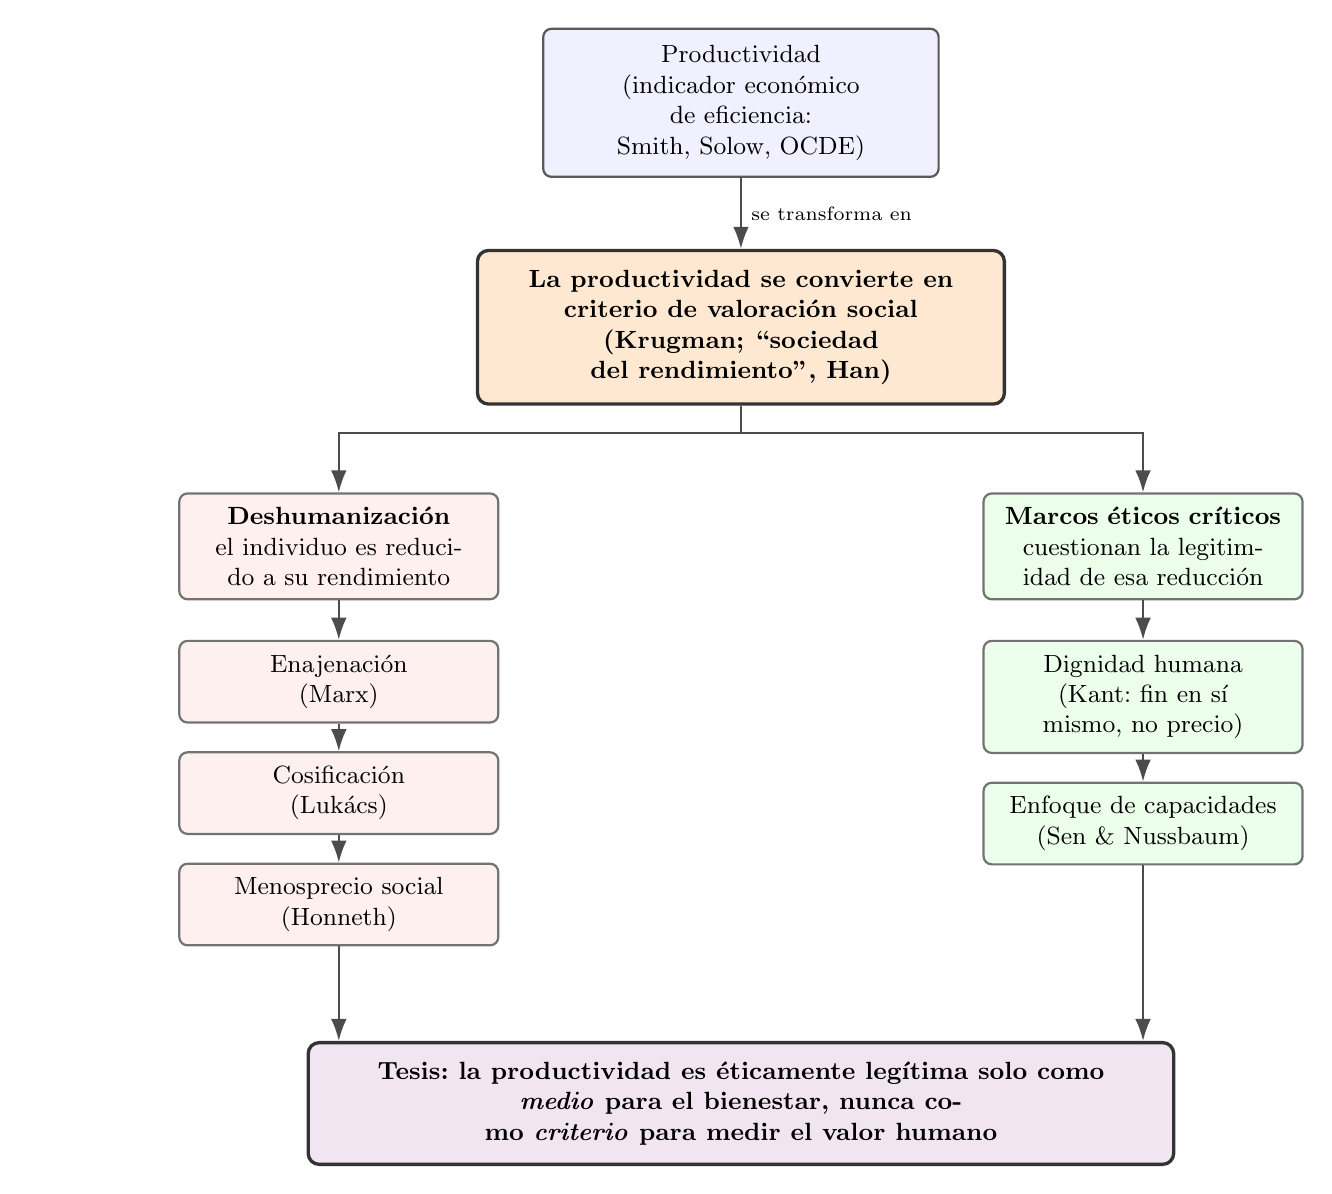
\begin{tikzpicture}[
        node distance=0.9cm and 1.4cm,
        every node/.style={font=\small},
        box/.style={
            rectangle, rounded corners=3pt, draw=black!65, thick,
            fill=blue!6, text width=4.6cm, align=center,
            minimum height=1.05cm, inner sep=6pt
        },
        keybox/.style={
            rectangle, rounded corners=4pt, draw=black!80, very thick,
            fill=orange!18, text width=6.2cm, align=center,
            minimum height=1.2cm, inner sep=7pt, font=\small\bfseries
        },
        subbox/.style={
            rectangle, rounded corners=3pt, draw=black!55, thick,
            fill=red!6, text width=3.7cm, align=center,
            minimum height=1cm, inner sep=5pt
        },
        critbox/.style={
            rectangle, rounded corners=3pt, draw=black!55, thick,
            fill=green!8, text width=3.7cm, align=center,
            minimum height=1cm, inner sep=5pt
        },
        concl/.style={
            rectangle, rounded corners=4pt, draw=black!80, very thick,
            fill=violet!10, text width=10.5cm, align=center,
            minimum height=1.2cm, inner sep=7pt, font=\small\bfseries
        },
        lbl/.style={font=\scriptsize\itshape, text width=3.4cm, align=center},
        arr/.style={-{Latex[length=2.8mm, width=2mm]}, thick, draw=black!70}
        ]

    % --- Nivel 1: punto de partida ---
        \node[box] (indicador)
            {Productividad\\ \small (indicador económico de eficiencia:\\ Smith, Solow, OCDE)};

    % --- Nivel 2: la transformación (núcleo de la tesis) ---
        \node[keybox, below=of indicador] (criterio)
            {La productividad se convierte en\\ criterio de valoración social\\ \small (Krugman; ``sociedad del rendimiento'', Han)};

        \node[lbl, left=0.15cm of criterio, xshift=-1.9cm, yshift=1.6cm] (contexto) {};

        \draw[arr] (indicador) -- node[right, font=\scriptsize] {se transforma en} (criterio);

    % --- Nivel 3: dos ramas ---
        \node[subbox, below left=1.1cm and -0.3cm of criterio] (deshum)
            {\textbf{Deshumanización}\\ \small el individuo es reducido a su rendimiento};

        \node[critbox, below right=1.1cm and -0.3cm of criterio] (critica)
            {\textbf{Marcos éticos críticos}\\ \small cuestionan la legitimidad de esa reducción};

        \draw[arr] (criterio.south) -- ++(0,-0.35) -| (deshum.north);
        \draw[arr] (criterio.south) -- ++(0,-0.35) -| (critica.north);

    % --- Sub-nodos de la rama "deshumanización" ---
        \node[subbox, below=0.5cm of deshum, text width=3.7cm] (marx)
            {Enajenación\\ \small (Marx)};
        \node[subbox, below=0.35cm of marx, text width=3.7cm] (lukacs)
            {Cosificación\\ \small (Lukács)};
        \node[subbox, below=0.35cm of lukacs, text width=3.7cm] (honneth)
            {Menosprecio social\\ \small (Honneth)};

        \draw[arr] (deshum) -- (marx);
        \draw[arr] (marx) -- (lukacs);
        \draw[arr] (lukacs) -- (honneth);

    % --- Sub-nodos de la rama "marcos críticos" ---
        \node[critbox, below=0.5cm of critica, text width=3.7cm] (kant)
            {Dignidad humana\\ \small (Kant: fin en sí mismo, no precio)};
        \node[critbox, below=0.35cm of kant, text width=3.7cm] (capacidades)
            {Enfoque de capacidades\\ \small (Sen \& Nussbaum)};

        \draw[arr] (critica) -- (kant);
        \draw[arr] (kant) -- (capacidades);

    % --- Nivel 4: conclusión / tesis  ---
    % Colocamos la caja final usando su anchor=north (borde superior) 
    % como punto de referencia, y le damos un espacio limpio de 1.2cm 
    % por debajo del nodo más bajo (honneth). Centramos respecto a criterio.
        \node[concl, anchor=north, yshift=-1.2cm] (tesis) at (criterio.south |- honneth.south) 
            {Tesis: la productividad es éticamente legítima solo como\\ \emph{medio} para el bienestar, nunca como \emph{criterio} para medir el valor humano};

    % Conectamos las flechas verticalmente a la caja 'tesis'.
        \draw[arr] (honneth.south) -- (honneth.south |- tesis.north);
        \draw[arr] (capacidades.south) -- (capacidades.south |- tesis.north);

    \end{tikzpicture}} %
    \caption{Esquema del argumento central: de indicador económico a criterio de valoración social}
    \label{fig:esquema-argumento}
\end{figure}

% ============================================================
% II) PRODUCTIVIDAD COMO CRITERIO DE ÉXITO
% ============================================================
\section{Productividad como criterio de éxito en la sociedad contemporánea}

    \subsection{Concepto de productividad}

    Para analizar el impacto de la productividad en la sociedad contemporánea, primero es necesario delimitar su significado desde la teoría económica. En términos generales, la productividad se entiende como una medida de eficiencia que refleja la capacidad de una economía para transformar recursos o factores de producción (\textit{inputs}) en bienes y servicios (\textit{outputs}). Como señala la \citet{ocde2023}, este concepto no debe confundirse con el volumen de producción: mientras que la producción expresa la cantidad total de bienes y servicios generados, la productividad mide cuánto producto se obtiene por cada unidad de trabajo, capital u otro factor utilizado.

    Esta noción de eficiencia material es el resultado de una evolución teórica que tuvo inicio en la economía clásica. \citet{smith1958} sostuvo que la división del trabajo incrementa la riqueza al favorecer la especialización de los trabajadores, reducir el tiempo perdido entre tareas e incentivar la incorporación de mejoras técnicas. Desde esta perspectiva, la productividad se relaciona con la organización más eficiente del proceso productivo.

    Una de las formalizaciones más influyentes de este concepto es el modelo de crecimiento de \citet{solow1956}, en el cual la producción total depende del capital, el trabajo y un componente residual asociado al progreso tecnológico y a la eficiencia. De manera simplificada, este modelo puede representarse mediante una función de producción tipo Cobb-Douglas:

% ------------------------------------------------------------------
% ECUACIÓN 1: función de producción (Cobb-Douglas / modelo de Solow)
% Representa cómo el producto (Y) depende del progreso tecnológico (A),
% el capital (K) y el trabajo (L).
% ------------------------------------------------------------------
\begin{equation}
    Y = A \cdot K^{\alpha} L^{1-\alpha}
    \label{eq:cobb-douglas}
\end{equation}

En la Ecuación~\ref{eq:cobb-douglas}, $Y$ representa el producto total, $A$ el nivel de productividad total de los factores (o "residuo de Solow"), $K$ el capital, $L$ el trabajo, y $\alpha$ la elasticidad del producto respecto al capital. Este componente $A$ es, precisamente, lo que la literatura económica identifica como productividad en sentido estricto.

A partir de la Ecuación~\ref{eq:cobb-douglas}, es posible despejar el residuo de Solow, es decir, la parte del crecimiento que no se explica por la simple acumulación de capital y trabajo:

% ------------------------------------------------------------------
% ECUACIÓN 2: residuo de Solow (productividad total de los factores)
% ------------------------------------------------------------------
\begin{equation}
    A = \frac{Y}{K^{\alpha} L^{1-\alpha}}
    \label{eq:residuo-solow}
\end{equation}

La Ecuación~\ref{eq:residuo-solow} muestra que la productividad ($A$) no es observable de forma directa, sino que se calcula como un residuo: aquello que el crecimiento del producto no logra explicar la simple acumulación de factores.

Sobre esta base, la economía contemporánea considera a la productividad como uno de los principales determinantes del crecimiento económico y del nivel de vida. En palabras de \citet{krugman1990}, «la productividad no lo es todo, pero a largo plazo lo es casi todo», pues la capacidad de una sociedad para elevar sus ingresos depende, en gran medida, de producir más eficientemente. Así, la productividad deja de ser solo un indicador técnico y adquiere un lugar central dentro de las estrategias de desarrollo económico.

\subsection{La productividad como criterio de éxito y derivaciones (precios e ingreso)}

Sin embargo, cuando la productividad deja de ser únicamente un criterio económico y pasa a convertirse en un parámetro para valorar el éxito de las personas, surgen importantes implicancias éticas. Aunque la productividad nació como un concepto técnico para medir la eficiencia económica, en la actualidad también influye en la forma en que las personas y las sociedades son evaluadas. Si el desarrollo de un país depende de producir cada vez más eficientemente, como sostiene la economía ortodoxa, resulta comprensible que la productividad pase a asociarse con el éxito, el mérito y el progreso individual. En este sentido, un criterio originalmente económico comienza a adquirir un contenido normativo: no solo describe el funcionamiento de la economía, sino que también establece expectativas sobre cómo deberían comportarse las personas.

Esta lógica puede apreciarse en la conocida y ya mencionada afirmación de \citet{krugman1990}; «la productividad no lo es todo, pero a largo plazo lo es casi todo». Aunque el autor emplea esta idea para destacar la importancia de la productividad en el crecimiento económico, reconoce que las estrategias para incrementarla suelen implicar sacrificios presentes en nombre de beneficios futuros. De esta forma, la productividad ya no se percibe únicamente como un indicador económico, sino que comienza a asociarse con el esfuerzo constante, el mérito y el éxito individual.

Las implicancias de esta transformación trascienden el ámbito económico. \citet{han2012} sostiene que la sociedad contemporánea ha pasado de estar regida por la prohibición y el control externo, a una “sociedad del rendimiento”, donde el propio individuo internaliza la exigencia de producir y optimizarse de manera continua. En este escenario, la presión ya no proviene exclusivamente del empleador o de las instituciones, sino del propio sujeto, que busca aumentar constantemente su desempeño convencido de que ello depende únicamente de su esfuerzo personal. Como señala Han, esta forma de autoexplotación resulta especialmente eficaz porque suele experimentarse como una expresión de libertad y realización individual.

En consecuencia, la productividad se convierte en un criterio de reconocimiento social y de valoración personal. Cuando el rendimiento económico pasa a definir el éxito de los individuos, la productividad deja de ser un instrumento al servicio de las personas y comienza a convertirse en un parámetro mediante el cual ellas mismas son juzgadas.

\subsection{En el contexto peruano: trabajo e informalidad}

Esta transformación adquiere características particulares en el contexto peruano, donde la exigencia de productividad convive con elevados niveles de informalidad y precariedad laboral. De acuerdo con el \citet{inei2025}, alrededor del 70\% de la PEA Ocupada trabaja en empleos informales, mientras que este sector genera una proporción significativamente menor del PBI, tal como se resume en la Tabla~\ref{tab:informalidad}.
% ------------------------------------------------------------------
% TABLA 1: Informalidad laboral en el Perú
% Ajusta los valores numéricos según la fuente que finalmente utilices
% (INEI, 2025). Los valores aquí son ilustrativos del orden de magnitud
% mencionado en el ensayo.
% ------------------------------------------------------------------
\begin{table}[H]
    \centering
    \caption{Empleo informal y aporte al PBI en el Perú (2024)}
    \label{tab:informalidad}
    \begin{tabular}{lcc}
        \toprule
        \textbf{Indicador} & \textbf{Sector informal} & \textbf{Sector formal} \\
        \midrule
        Participación en el empleo total & 55,7\% & 44,3\% \\
        Aporte al PBI                    & 19\% & 81\% \\
        Acceso a protección social       & Bajo   & Alto   \\
        \bottomrule
    \end{tabular}

    \vspace{0.2cm}
    \footnotesize{\textit{Nota.} Elaboración propia con base en \citet{inei2025}.}
\end{table}

Como se observa en la Tabla~\ref{tab:informalidad}, el sector informal genera 55,7\% del empleo de la economía pero solamente 19\% del PBI, lo que permite discutir la baja productividad relativa y cuestionar que la productividad pueda utilizarse como medida del valor social de las personas. El \citet{mtpe2026} identifica como causas de la informalidad la escasa diversificación productiva, las brechas de capital humano y el limitado acceso a mecanismos de protección social. En estas condiciones, el autoempleo y otras formas de trabajo informal constituyen, con frecuencia, estrategias de subsistencia antes que decisiones plenamente voluntarias. En este sentido, \citet{carbonetto1988} sostienen que una parte importante de los trabajadores termina «inventando» ocupaciones de supervivencia debido a la incapacidad del sector moderno para absorber la mano de obra disponible. En consecuencia, exigir mayores niveles de productividad sin modificar dichas condiciones implica trasladar al trabajador la responsabilidad de superar obstáculos cuya naturaleza es principalmente estructural.

Esta tensión se intensifica ante los procesos de cambio tecnológico. Como advierte la \citet{oit2026}, cuando las instituciones laborales y los sistemas de protección social son débiles, la incorporación de nuevas tecnologías puede profundizar la desigualdad y ampliar la informalidad en lugar de favorecer un desarrollo más inclusivo (\citet{bertranou2026}). En este contexto, la «sociedad del rendimiento» descrita por \citet{han2012} adquiere características particulares: la exigencia de ser permanentemente productivo deja de responder únicamente a una aspiración de éxito personal y se convierte en una estrategia de supervivencia. De este modo, la presión por rendir no elimina las limitaciones estructurales del mercado laboral peruano, sino que desplaza sus consecuencias hacia el individuo, quien termina asumiendo como un fracaso personal aquello que, en gran medida, constituye el resultado de condiciones económicas y sociales que escapan de su control. 

En consecuencia, el discurso de la productividad termina asociando el éxito económico con el mérito individual, aun cuando las oportunidades para desarrollar dicho mérito se encuentran profundamente condicionadas por factores estructurales. Así, quienes no alcanzan determinados niveles de rendimiento corren el riesgo de ser percibidos —y de percibirse a sí mismos— como menos valiosos, desplazando hacia el individuo la responsabilidad por desigualdades cuya raíz es, en gran medida, social y económica.

Como se aprecia en el Apéndice~\ref{apendice:A} (ver Figura~\ref{fig:participacion}), la informalidad mantiene una participación relativamente constante en el producto interno bruto peruano, con un promedio cercano al 18,5\% entre 2007 y 2024. Este comportamiento evidencia que, pese a los avances normativos y tecnológicos, la estructura productiva nacional continúa sustentándose en una base informal persistente. Según el \citet{inei2025}, esta estabilidad refleja la limitada capacidad del sector formal para absorber la fuerza laboral y la permanencia de actividades de baja productividad. En este sentido, el gráfico no solo ilustra una tendencia económica, sino también una manifestación cuantitativa de las restricciones estructurales que condicionan el mercado laboral peruano y que, como se argumenta en el texto, trasladan al individuo la carga de una desigualdad que tiene raíces sistémicas.

% ============================================================
% III) IMPLICANCIAS ÉTICAS
% ============================================================

\section{Implicancias éticas de la productividad como criterio de valoración social}

    \subsection{La productividad como criterio de valoración y la deshumanización del individuo}

Cuando la productividad deja de ser un indicador económico y se convierte en el principal criterio para valorar a las personas, el trabajo deja de ser únicamente una actividad productiva y pasa a definir el valor social del individuo. \citet{marx1968} sostiene que, bajo determinadas relaciones de producción, el trabajador experimenta un proceso de enajenación en el que el trabajo deja de ser una expresión de su humanidad para convertirse en un medio de subsistencia. En estas condiciones, el producto de su trabajo se le enfrenta como algo ajeno, mientras que su propia actividad deja de realizarlo y pasa a negarlo. En lugar de desarrollar libremente sus capacidades, el individuo termina subordinando su vida a las exigencias de la producción, hasta el punto de encontrar mayor libertad fuera del trabajo que en él. Cuando el valor de una persona depende principalmente de su productividad, esta lógica de enajenación se profundiza, pues el individuo comienza a definirse por el rendimiento que es capaz de ofrecer y no por su dignidad inherente.

\citet{lukacs1970} amplía este diagnóstico mediante el concepto de cosificación. Según el autor, cuando predominan los criterios de cálculo y eficiencia, las relaciones sociales adquieren la apariencia de relaciones entre cosas y las capacidades humanas pasan a tratarse como recursos cuantificables. El trabajador deja de ser el sujeto del proceso productivo para convertirse en una pieza funcional dentro de un sistema guiado por el rendimiento. De este modo, la productividad ya no representa únicamente una herramienta para organizar la producción, sino un criterio que transforma las cualidades humanas en variables susceptibles de medición, comparación y evaluación.

Las consecuencias de este proceso también se manifiestan en el plano del reconocimiento social. \cite{honneth1997} sostiene que la autoestima de las personas depende, en buena medida, del reconocimiento que reciben de los demás. Sin embargo, cuando dicho reconocimiento se vincula casi exclusivamente al rendimiento económico, el valor social del individuo pasa a medirse por su capacidad de producir. Quienes no alcanzan los niveles de productividad socialmente esperados pueden experimentar formas de menosprecio que afectan su autoestima y generan sentimientos de vergüenza o fracaso, aun cuando sus limitaciones respondan a condiciones estructurales y no únicamente a decisiones individuales.

En suma, estos enfoques muestran que el problema ético no radica en la productividad como herramienta para mejorar la eficiencia económica, sino en su transformación en un criterio para determinar el valor de las personas. Cuando el reconocimiento social depende principalmente del rendimiento, el individuo deja de ser apreciado por su dignidad inherente y comienza a ser valorado por aquello que produce. La Figura~\ref{fig:esquema-deshumanizacion} sintetiza estas tres etapas como un proceso progresivo: cada una profundiza la anterior, hasta desembocar en la reducción de la persona a su capacidad de generar rendimiento.

% ------------------------------------------------------------------
\begin{figure}[H]
    \centering
    \scalebox{0.9}{%
    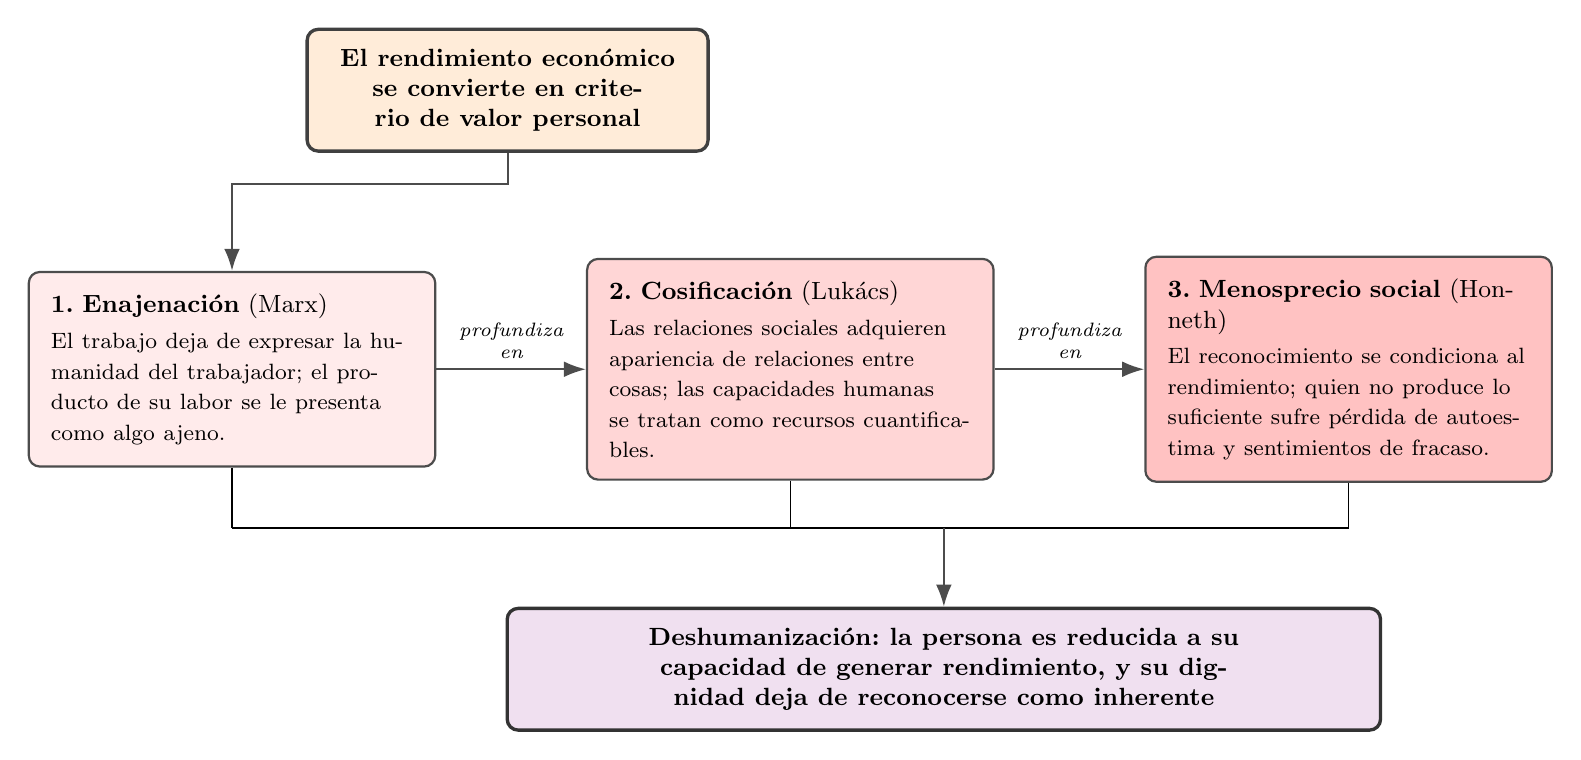
\begin{tikzpicture}[
        node distance=1.5cm,
        every node/.style={font=\small},
        etapa/.style={
            rectangle, rounded corners=4pt, draw=black!70, thick,
            text width=4.6cm, align=left, minimum height=2.15cm, inner sep=8pt
        },
        origen/.style={
            rectangle, rounded corners=4pt, draw=black!75, very thick,
            fill=orange!15, text width=4.6cm, align=center,
            minimum height=1.3cm, inner sep=7pt, font=\small\bfseries
        },
        destino/.style={
            rectangle, rounded corners=4pt, draw=black!80, very thick,
            fill=violet!12, text width=10.6cm, align=center,
            minimum height=1.3cm, inner sep=7pt, font=\small\bfseries
        },
        arr/.style={-{Latex[length=2.8mm, width=2mm]}, thick, draw=black!70}
    ]

% --- Punto de partida ---
        \node[origen] (inicio)
            {El rendimiento económico se convierte en criterio de valor personal};

% --- Etapa 1: Enajenación (Marx) ---
        \node[etapa, fill=red!8, below=1.5cm of inicio, xshift=-3.5cm] (marx)
            {\textbf{1. Enajenación} \small(Marx)\\[2pt]
            \footnotesize El trabajo deja de expresar la humanidad del trabajador; el producto de su labor se le presenta como algo ajeno.};

% --- Etapa 2: Cosificación (Lukács) ---
        \node[etapa, fill=red!16, right=1.9cm of marx] (lukacs)
            {\textbf{2. Cosificación} \small(Lukács)\\[2pt]
            \footnotesize Las relaciones sociales adquieren apariencia de relaciones entre cosas; las capacidades humanas se tratan como recursos cuantificables.};

% --- Etapa 3: Menosprecio social (Honneth) ---
        \node[etapa, fill=red!24, right=1.9cm of lukacs] (honneth)
            {\textbf{3. Menosprecio social} \small(Honneth)\\[2pt]
            \footnotesize El reconocimiento se condiciona al rendimiento; quien no produce lo suficiente sufre pérdida de autoestima y sentimientos de fracaso.};

% --- Flechas de secuencia (profundización progresiva) ---
        \draw[arr] (inicio.south) -- ++(0,-0.4) -| (marx.north);
        \draw[arr] (marx.east) -- node[above, font=\scriptsize\itshape, text width=1.5cm, align=center] {profundiza en} (lukacs.west);
        \draw[arr] (lukacs.east) -- node[above, font=\scriptsize\itshape, text width=1.5cm, align=center] {profundiza en} (honneth.west);

%--------- --- Resultado final -------------------
        \node[destino, below=1.6cm of lukacs, xshift=1.95cm] (resultado)
            {Deshumanización: la persona es reducida a su capacidad de generar rendimiento, y su dignidad deja de reconocerse como inherente};

        \path (lukacs.south) ++(0,-0.6) coordinate (nivel_linea);

        \draw (marx.south) -- (marx.south |- nivel_linea);
        \draw (lukacs.south) -- (lukacs.south |- nivel_linea);
        \draw (honneth.south) -- (honneth.south |- nivel_linea);

        \draw (marx.south |- nivel_linea) -- (honneth.south |- nivel_linea);

        \draw[arr] (resultado.north |- nivel_linea) -- (resultado.north);
    \end{tikzpicture}} %
    
    \caption{Proceso de deshumanización a partir del criterio de rendimiento}
    \label{fig:esquema-deshumanizacion}
\end{figure}

\subsection{Evaluación ética desde la dignidad humana y el enfoque de las capacidades}

Si la productividad se convierte en el principal criterio para valorar a las personas, surge una cuestión ética fundamental: ¿es legítimo que el rendimiento económico determine el valor de un ser humano? Desde la deontología kantiana, la respuesta es negativa.
En la Fundamentación de la metafísica de las costumbres, \cite{kant1996} distingue entre aquello que tiene precio y aquello que posee dignidad. Mientras las cosas pueden ser sustituidas por un equivalente, las personas poseen un valor intrínseco que no admite comparación ni intercambio. Por ello, el imperativo categórico exige tratar a toda persona siempre como un fin en sí misma y nunca únicamente como un medio para alcanzar otros fines.

Desde esta perspectiva, valorar a los individuos exclusivamente por su productividad implica reducirlos a instrumentos para la generación de riqueza o eficiencia económica. El problema ético no reside en promover la productividad como objetivo económico, sino en convertirla en la medida del valor humano. Cuando el reconocimiento social depende principalmente del rendimiento, la dignidad deja de ser reconocida como un atributo inherente a toda persona y pasa a condicionarse por su utilidad económica, contradiciendo el principio kantiano de respetar a cada individuo como un fin en sí mismo.

Esta crítica también encuentra respaldo en el enfoque de las capacidades desarrollado por \citet{sen1999} y \citet{nussbaum2012}. Ambos autores sostienen que el bienestar y el desarrollo no deben evaluarse únicamente mediante indicadores económicos como el ingreso o la productividad, sino a partir de las oportunidades reales que poseen las personas para desarrollar las capacidades que valoran. Mientras Sen enfatiza la libertad sustantiva para elegir diferentes formas de vida, Nussbaum propone un conjunto de capacidades centrales —como la salud, la integridad física y la razón práctica— que constituyen las condiciones mínimas para una vida digna.

En consecuencia, medir el valor de una persona exclusivamente por su rendimiento económico invisibiliza las desigualdades en las oportunidades y desconoce dimensiones fundamentales de la vida humana que no pueden reducirse a criterios de eficiencia. Desde estos enfoques, el desarrollo debe orientarse a ampliar las capacidades y proteger la dignidad de las personas, en lugar de valorar su existencia únicamente por aquello que producen. Desde esta perspectiva, una sociedad que reduce el valor de las personas a su productividad no solo incurre en un problema ético, sino que también puede generar efectos concretos sobre su bienestar y calidad de vida. 

En el contexto peruano, \citet{valdivieso2025} señala que alrededor del 70 \% de los trabajadores experimenta estrés crónico y que uno de cada seis presenta síndrome de burnout. Asimismo, \citet{condori2026} recopilan otros estudios nacionales que reportan elevados niveles de agotamiento laboral. Aunque estos resultados no pueden atribuirse exclusivamente a la exigencia de productividad, evidencian que las dinámicas de presión permanente por el rendimiento pueden afectar significativamente el bienestar psicológico de las personas. En este sentido, el burnout constituye una manifestación concreta de las formas de autoexplotación, enajenación y cosificación analizadas previamente, al mostrar cómo la presión constante por rendir puede deteriorar la salud física y mental de los trabajadores.

% ============================================================
% IV) CONCLUSIÓN
% ============================================================
\section{Conclusión}

La productividad constituye uno de los pilares del desarrollo económico moderno. Sin embargo, el análisis desarrollado en este ensayo muestra que el problema ético no reside en la productividad en sí misma (Ecuaciones~\ref{eq:cobb-douglas} y \ref{eq:residuo-solow}), sino en su transformación en el principal criterio para valorar a las personas. Cuando el rendimiento económico deja de ser un instrumento para promover el bienestar colectivo y pasa a definir el mérito, el reconocimiento social y el valor individual, se produce una reducción de la persona a su utilidad económica.

El caso peruano, resumido en la Tabla~\ref{tab:informalidad}, revela con particular claridad las limitaciones de una visión centrada exclusivamente en el rendimiento: atribuir el éxito o el fracaso únicamente al esfuerzo individual invisibiliza las desigualdades estructurales que condicionan las oportunidades de millones de trabajadores. Asimismo, la evidencia sobre el incremento del estrés y el síndrome de burnout muestra que la presión permanente por responder a exigencias de rendimiento puede tener consecuencias que trascienden el ámbito económico y afectan directamente el bienestar y la salud mental.

En consecuencia, una sociedad comprometida con el desarrollo no debería limitarse a incrementar la productividad, sino también preguntarse al servicio de quién se encuentra ese crecimiento y en qué condiciones se alcanza. Promover economías más productivas constituye un objetivo legítimo; sin embargo, dicho propósito solo resulta éticamente aceptable cuando la productividad permanece como un medio para mejorar la vida de las personas y no cuando se convierte en el criterio mediante el cual ellas son juzgadas. En última instancia, el verdadero desarrollo consiste en construir una sociedad donde la eficiencia económica sea compatible con el reconocimiento de la dignidad inherente de toda persona.

% ==========================================
% BIBLIOGRAFÍA
% ==========================================
\bibliographystyle{apacite}
\bibliography{references}

% ==========================================
% APÉNDICES
% ==========================================
\appendix
    \section{Datos estadísticos complementarios}
\label{apendice:A}

El siguiente gráfico detalla la evolución y el impacto económico del sector informal mencionado en la Sección 2.3 del presente ensayo.

\begin{figure}[H]
    \centering
    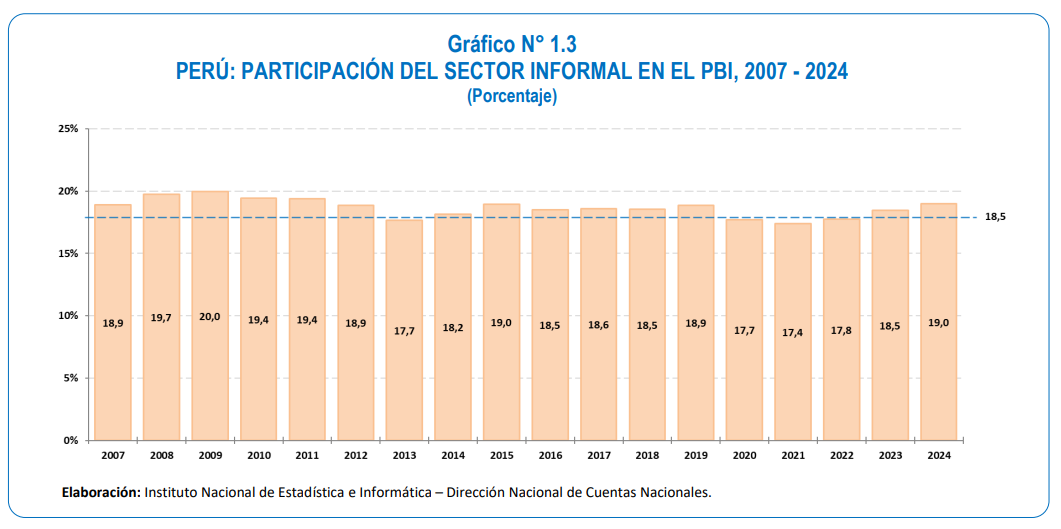
\includegraphics[width=0.7\textwidth]{imagenes/participación informal pbi.png}
    \caption{Perú: Participación del sector informal en el PBI, 2007-2024. Fuente: \citet{inei2025}}
    \label{fig:participacion}
\end{figure}

\end{document}